\begin{equation}
    \begin{gathered}
        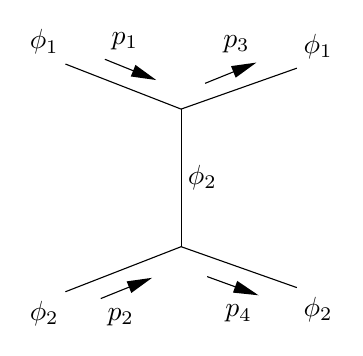
\begin{tikzpicture}[x=0.75pt,y=0.75pt,yscale=-1,xscale=1]
            %uncomment if require: \path (0,300); %set diagram left start at 0, and has height of 300
            
            %Straight Lines [id:da3658497276365975] 
            \draw    (299.45,102.74) -- (243.71,122.45) ;
            %Straight Lines [id:da1392939324999145] 
            \draw    (187.97,100.74) -- (243.71,122.45) ;
            %Straight Lines [id:da5792004960946098] 
            \draw    (206.98,98.45) -- (229.85,107.7) ;
            \draw [shift={(231.71,108.45)}, rotate = 202.02] [fill={rgb, 255:red, 0; green, 0; blue, 0 }  ][line width=0.08]  [draw opacity=0] (12,-3) -- (0,0) -- (12,3) -- cycle    ;
            %Straight Lines [id:da5743221216400951] 
            \draw    (278.14,100.78) -- (255.27,110.03) ;
            \draw [shift={(279.99,100.03)}, rotate = 157.98] [fill={rgb, 255:red, 0; green, 0; blue, 0 }  ][line width=0.08]  [draw opacity=0] (12,-3) -- (0,0) -- (12,3) -- cycle    ;
            %Straight Lines [id:da927376856169188] 
            \draw    (243.71,122.45) -- (243.71,188.74) ;
            %Straight Lines [id:da8947002419253893] 
            \draw    (299.45,208.45) -- (243.71,188.74) ;
            %Straight Lines [id:da2196394430244235] 
            \draw    (187.97,210.45) -- (243.71,188.74) ;
            %Straight Lines [id:da06264839191963989] 
            \draw    (204.98,213.74) -- (227.85,204.49) ;
            \draw [shift={(229.71,203.74)}, rotate = 517.98] [fill={rgb, 255:red, 0; green, 0; blue, 0 }  ][line width=0.08]  [draw opacity=0] (12,-3) -- (0,0) -- (12,3) -- cycle    ;
            %Straight Lines [id:da7986552586213247] 
            \draw    (279.11,211.47) -- (256.27,203.15) ;
            \draw [shift={(280.99,212.15)}, rotate = 200] [fill={rgb, 255:red, 0; green, 0; blue, 0 }  ][line width=0.08]  [draw opacity=0] (12,-3) -- (0,0) -- (12,3) -- cycle    ;
            
            % Text Node
            \draw (185.97,97.34) node [anchor=south east] [inner sep=0.75pt]    {$\phi _{1}$};
            % Text Node
            \draw (185.97,213.85) node [anchor=north east] [inner sep=0.75pt]    {$\phi _{2}$};
            % Text Node
            \draw (208.98,95.05) node [anchor=south west] [inner sep=0.75pt]    {$p_{1}$};
            % Text Node
            \draw (206.98,217.14) node [anchor=north west][inner sep=0.75pt]    {$p_{2}$};
            % Text Node
            \draw (245.71,155.59) node [anchor=west] [inner sep=0.75pt]    {$\phi _{2}$};
            % Text Node
            \draw (277.99,96.63) node [anchor=south east] [inner sep=0.75pt]    {$p_{3}$};
            % Text Node
            \draw (278.99,215.55) node [anchor=north east] [inner sep=0.75pt]    {$p_{4}$};
            % Text Node
            \draw (301.45,99.34) node [anchor=south west] [inner sep=0.75pt]    {$\phi _{1}$};
            % Text Node
            \draw (301.45,211.85) node [anchor=north west][inner sep=0.75pt]    {$\phi _{2}$};
            \end{tikzpicture}            
    \end{gathered} \quad 
    \begin{aligned}[t]
         &\eqqcolon \ii \mathcal{M}_{t2} = \frac{\ii}{(p_1 - p_3)^2 + \ii 0^+} (- \ii \lambda p_3 \cdot (p_1 - p_3)) ( \ii \lambda (p_1 - p_3) \cdot p_4) \\
         &= \ii \frac{\lambda^2 (p_3 \cdot (p_1 - p_3))((p_1 - p_3) \cdot p_4)}{t + \ii 0^+ },
    \end{aligned}
\end{equation}